% !TeX program = pdfLaTeX
\documentclass[12pt]{article}
\usepackage{amsmath}
\usepackage{graphicx,psfrag,epsf}
\usepackage{enumerate}
\usepackage{natbib}
\usepackage{textcomp}
\usepackage[hyphens]{url} % not crucial - just used below for the URL
\usepackage{hyperref}
\providecommand{\tightlist}{%
  \setlength{\itemsep}{0pt}\setlength{\parskip}{0pt}}

%\pdfminorversion=4
% NOTE: To produce blinded version, replace "0" with "1" below.
\newcommand{\blind}{0}

% DON'T change margins - should be 1 inch all around.
\addtolength{\oddsidemargin}{-.5in}%
\addtolength{\evensidemargin}{-.5in}%
\addtolength{\textwidth}{1in}%
\addtolength{\textheight}{1.3in}%
\addtolength{\topmargin}{-.8in}%

%% load any required packages here




\begin{document}


\def\spacingset#1{\renewcommand{\baselinestretch}%
{#1}\small\normalsize} \spacingset{1}


%%%%%%%%%%%%%%%%%%%%%%%%%%%%%%%%%%%%%%%%%%%%%%%%%%%%%%%%%%%%%%%%%%%%%%%%%%%%%%

\if0\blind
{
  \title{\bf Can a deep learning model read residual plots?}

  \author{
        Author 1 \thanks{The authors gratefully acknowledge \ldots{}} \\
    Department of YYY, University of XXX\\
     and \\     Author 2 \\
    Department of ZZZ, University of WWW\\
      }
  \maketitle
} \fi

\if1\blind
{
  \bigskip
  \bigskip
  \bigskip
  \begin{center}
    {\LARGE\bf Can a deep learning model read residual plots?}
  \end{center}
  \medskip
} \fi

\bigskip
\begin{abstract}
Residuals plots are a primary means to diagnose statistical models. It
requires human evaluation to determine if the structure in the plot is
consistent with a random variation or not. If not, then the diagnosis is
that the model has not adequately captured the relationships between
response and explanatory variable in the data. This thesis develops a
computer vision model to read residual plots. It compares results with a
large database of human evaluations. The evaluations were conducted
using a protocol called the ``lineup'' which places residual plots in a
formal framework for statistical hypothesis testing. The comparison
between computer and human is made on a very restricted and controlled
set of residual plot structures. A new small human subject study is also
conducted to compare human vs.~computer in reading heteroscedasticity.
\end{abstract}

\noindent%
{\it Keywords:} 3 to 6 keywords, that do not appear in the title
\vfill

\newpage
\spacingset{1.45} % DON'T change the spacing!

\section{Introduction}\label{introduction}

``The multiple regression model for cross-sectional data is still the
most widely used vehicle for empirical analysis in economics and other
social sciences'' \citep{IE17}. Detecting possible violations of the
Gauss-Markov assumptions is crucial to interpreting the data properly,
especially in the early stage of analysis.\citep{zeileis2002} There are
several distribution tests that are commonly used, for instance, the
Pearson correlation test for detecting linear relationship; the
Breusch-Pagan test and White test for investigating heteroskedasticity.
But primarily residual plots are the main diagnostic tool and these rely
on human evaluation. Because data plots show a lot more information than
a single statistic. A good example here would be Anscombe's Quartet.
``It is a set of four distinct data sets each consisting of 11 (x,y)
pairs where each dataset produces the same summary statistics (mean,
standard deviation, and correlation) while producing vastly different
plots'' \citep{ANS73}. Matejka and Fitzmaurice also did an interesting
study on this issue, they used `datasaurus' data from \citet{DS16} and
generated a series of data with same statistics but very different plots
as shown in figure \ref{fig:saurus}. \citep{JM17}

\begin{figure}
\centering
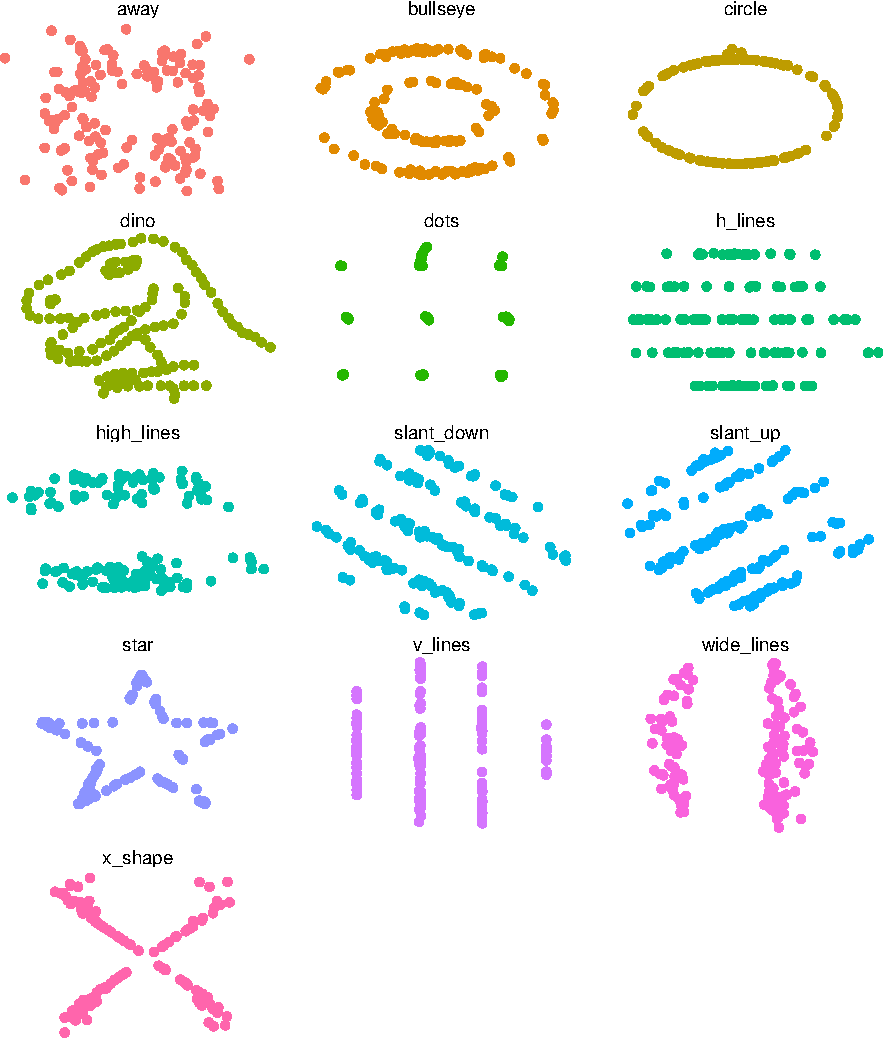
\includegraphics{pc_plots_files/figure-latex/saurus-1.pdf}
\caption{Each dataset has the same summary statistics to two decimal
places: (E(x)=54.26, E(y)=47.83, Pearson's r=, sd(x)=16.76, sd(y)=26.93}
\end{figure}

\section{Experimental Methods}
\label{sec:experiment}

Former studies have shown that human eyes are sensitive to the
systematic patterns in data plots. With proper manipulation, visualized
plots can be used as test statistics and perform a valid hypothesis
test. One example of these protocols that provides inferential validity
is called ``lineup'' which is introduced by \citet{HW10}. ``The protocol
consists of generating 19 null plots (could be other numbers), inserting
the plot of the real data in a random location among the null plots and
asking the human viewer to single out one of the 20 plots as most
different from the others'' \citep{HW10}. If the real plot is chosen, it
means the real data is likely to be different from the null hypothesis,
so we reject the null hypothesis with 5\% chance to be wrong (Type I
error). Because if all 20 plots are generated from the null
distribution, the chance of one plot being picked is \(1/20\) which is
5\%. With the assistance of ``lineup'', we avoid falling into the trap
of apophenia where we see patterns in random noise. This protocol has
proved to be valid and powerful theoretically as well as practically
through human experiments, especially when the assumptions for doing
conventional tests are violated \citep{MM13}. The human factors that may
influence visual statistical inference were also investigated by
\citet{human2014}. The experiments in \citet{human2014} suggest that
``individual skills vary substantially, but demographics do not have a
huge effect on performance.'' Although there are some statistically
significant factors such as ``having a graduate degree'' and ``living
country'', the effects of these factors are minimal. These results
demonstrate the robustness of the test against different human factors.
Figure \ref{fig:lineup} is an example of the lineup. Which plot do you
think is the most different? If you choose plot one, we are 95\%
confident to reject the no-relationship assumption between the two
variables, ``hp'' and ``disp'' \citep{SIM18}. The lineup protocol can
also be used for other types of testing by choosing different types of
plot. For example, normality can be tested using QQ plot; the difference
in mean can be tested using box plot; etc.

The question that arises today is whether we can train a computer to
read residual plot and make relevant decisions, particularly with a
computer vision approach such as deep learning. If this is feasible, we
can have the deep learning model process a lot more data than a human
can manage. Thus, the cost of rendering visual inference will become
much lower.

\begin{figure}
\centering
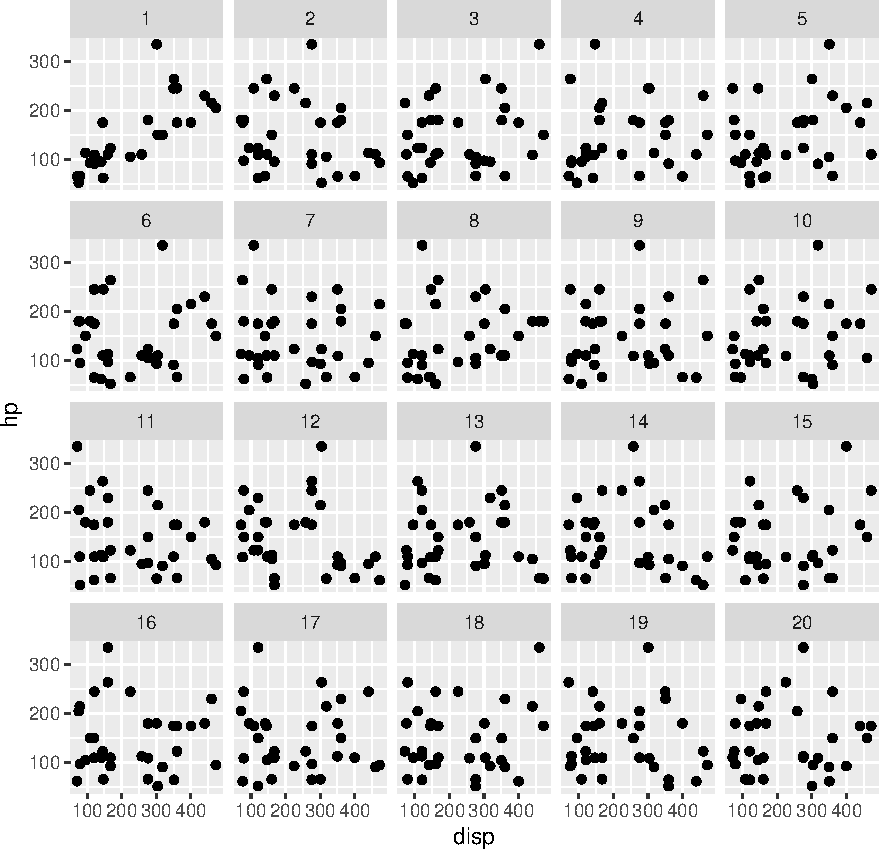
\includegraphics{pc_plots_files/figure-latex/lineup-1.pdf}
\caption{Scatterplot lineup example: one plot is the data, the rest are
generated from a null model assuming no relationship between the two
variables. In this lineup it is easy to see that plot 1, which is the
data plot, is different from the rest.}
\end{figure}

The motivation for the task is provided in a blog post by Giora Simchoni
\citep{SIM18}. He has designed a deep learning model to test the
significance of the linear relationship between two variables for
samples of size 50. The model reached over 93\% accuracy on unseen test
data. He also mentioned that the computer fails to pick up a strong
non-linear relationship even though the Pearson'r is as high as -0.84
\citep{SIM18}. So the short conclusion is the computer vision is not
perfect, in that it is not as flexible as human vision. As Simchoni
explained in his article, the model can only distinguish linear
relationship from no-relationship as trained. However, we think this
fact is just another example reflecting the importance of visualization
as we discussed above. A strong correlation does not necessarily mean a
linear relationship. We should always refer to the plot before making
any statement. What's more, if we want the model to be more flexible, we
could simply adjust our design of training accordingly. Therefore, in
this article, we are trying to further Simchoni's study. More
specifically, we will build two computer models to perform two
hypothesis tests as follows. The first hypothesis test is:

\(H_0\): There are no relationships between the two variables.

\(H_1\): There is a linear relationship between the two variables where
all Gauss-Markov assumptions are met.

The second hypothesis test is:

\(H_0\): There is a linear relationship between the two variables where
all Gauss-Markov assumptions are met.

\(H_1\): There is a linear relationship between the two variables where
the variance of the error term is not a constant while all other
Gauss-Markov assumptions are met.

For ease of exposition, only the regression model with one explanatory
variable will be considered in this paper, but many of the results can
be generalized to other cases including multiple regression model.
Because the ``statistics'' we will use is the scatterplot, in terms of
teaching the computer reading the plot, one variable is enough to
generate different patterns in that plot for convnets to learn. And this
makes the design process much simpler.

The model we will use is the convolutional neural networks, also known
as convnets, a type of deep-learning model ``almost universally used in
computer vision applications'' \citep{DLR18}. The very first
convolutional neural networks, called the ``LeNet5'' which was born in
1994, propelled the field of deep learning. However, this technique was
in incubation from 1998 to 2010. In recent years, with the increasing
data availability and more advanced technology, the design of the neural
network architecture became more and more successful. Many types of
neural network architectures have been developed since then, such as the
``Dan Ciresan Net'' which enabled the implementation of GPU for the
first time, and the ``AlexNet'' which used the so-called ``ReLU''
function as the activation function and started a small revolution in
the deep learning world, etc. \citep{cnn2017} Basically convolutional
neural networks has two interesting properties: ``the patterns they
learn are translation invariant'', and ``they can learn spatial
hierarchies of patterns'' \citep{DLR18}. The first property implies that
once the model learns how to recognize linear/heteroskedasticity
patterns, it can detect those patterns regardless of their direction,
thus handling negative/positive relationship automatically in our case.

Unlike the classical programming where human input rules, in deep
learning paradigm, we provide data and the answers associated with the
data. Deep learning algorithm will output the rules, and these rules can
then be used on new data to make predictions. To make our life easier,
we can also think of the deep learning neural network as a complex
nonlinear model which could estimate millions of parameters
(\(\textbf{w}\)) with a big enough dataset. As usual regression problem,
to get the estimates of unknown parameters (\(\textbf{w}\)), we need to
provide the model with the dependent variable (\(y_i\)) and the
independent variables (\(\textbf{x}_i\)). In this case, the independent
variable will be the images of data plots (in forms of matrices)
simulated from the null distribution and the alternative distribution,
and dependent variable will be the labels of that plot indicating the
true relationship of the original data. Once we have the estimated
parameters (\(\hat{\textbf{w}}\)), we then can use them to classify
unseen data plots, e.g.~to perform a hypothesis test.

The architecture used in this study is a fundamental one. The estimation
method for the deep-learning model is called ``backpropagation''
algorithm which is a way to train chains of parametric operations using
gradient-descent optimization. The gradient-descent optimizer is meant
to find the set of parameters such that the cost function reaches its
minimum. The form of the cost functions or loss function is determined
per each question. In both two experiments conducted in this paper, the
deep learning model is expected to complete binary classification task,
e.g.~tell ``linearly correlated'' variables from ``independent''
variables for the first experiment, tell ``heteroskedasticity errors''
from ``normal errors'' for the second experiment. As introduced by
\citet{DLR18}, ``crossentropy is usually the best choice (as the loss
function) when you're dealing with models that output probabilities''.
Originated from Information Theory, crossentropy is a quantity measuring
the distance between probability distributions. In deep learning world,
it measures the distance between the true distribution and the
predictions. Therefore, in this paper, the binary crossentropy loss
function will be used. The associated cost function is of the form,
\[J(\textbf{w})=- \frac{1}{N}\sum_{i=1}^N\left(  
\ y_i\ log\hat{y_i}+(1-y_i)\ log(1-\hat{y_i})  
\right)\] where
\(\hat{y_i} = g(\textbf{w} \times \textbf{x}_i) = \frac{1}{1+e^{-\textbf{w} \times \textbf{x}_i}}\)
and \(g(z)\) is the logistic function.

\section{Results}
\label{sec:results}

The main procedures involved in constructing and selecting a convnets
model are shown in figure \ref{dgpc}. The convnets is trained on
``train'' and ``validation'' set. A certain number of iterations over
all samples are done, the fitted convnets given by each iteration are
saved, one best model is chosen as the representative for the computer
according to the overall accuracy on the unseen ``test'' set.

The main procedures of the human evaluating lineup are given in figure
\ref{dghm}. ``Real data'' and ``null data'' stand for datasets simulated
under the alternative hypothesis and the null hypothesis respectively.
More detailed procedures relating each hypothesis test are described in
chapter 2 and chapter 3.

Chapter 2 compares computer performance against the database of human
evaluation in reading linear relationship. Steps of constructing
computer experiment are discussed, Turk study is explained, the
comparison results are given. Chapter 3 compares computer performance
against the results from the new human subject study. Details of this
new human subject study are provided. A white-test \citep{white} for
testing heteroskedasticity is introduced. The comparing results between
the human, the computer and the white test are presented. Chapter 4
contains a short summary and some discussion regarding the future study.

\begin{figure*}[h]
\centerline{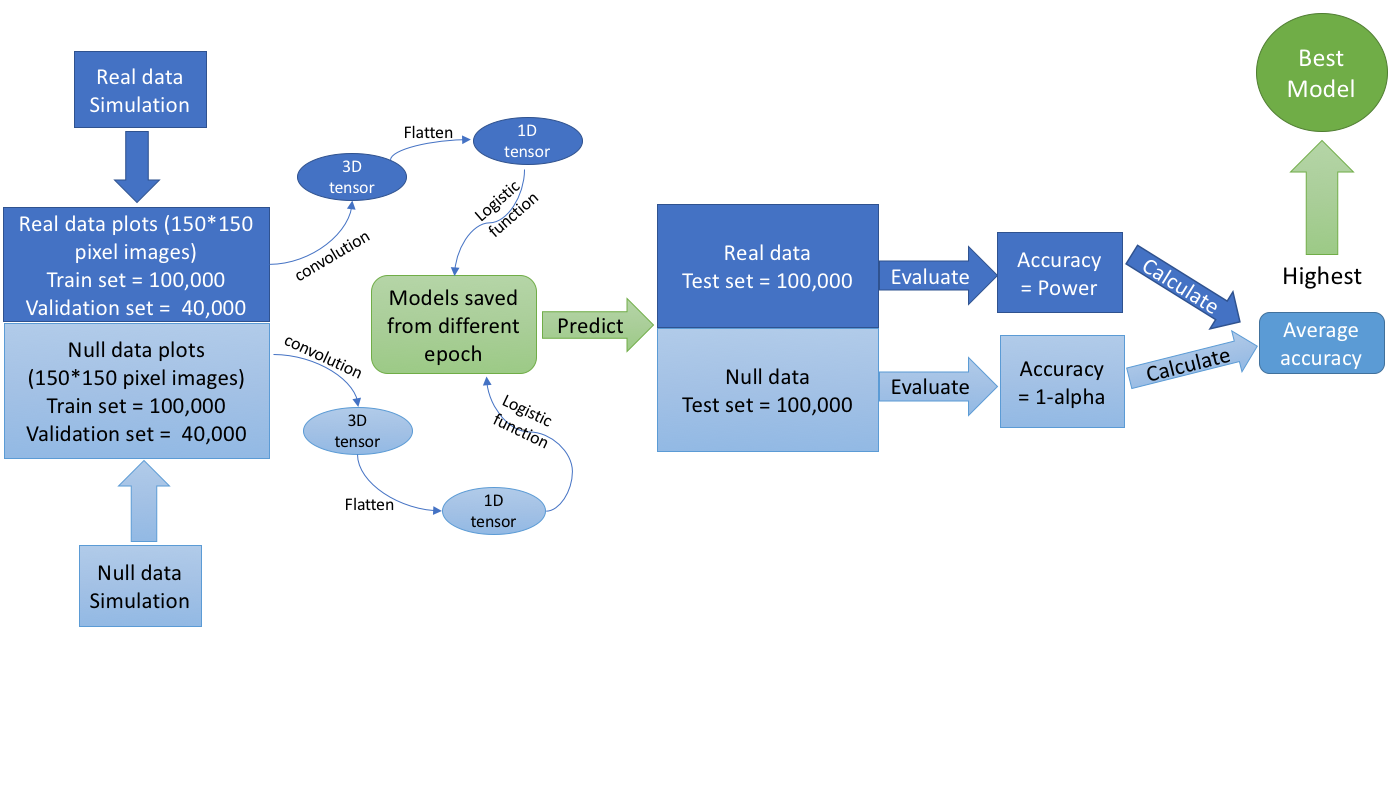
\includegraphics[width=15cm]{figures/diagpc.png}}
\caption{Diagram illustrating the training, diagnosis and choice of the computer model. Based on 480,000 simulated data sets used to create $150\times 150$ pixel images, divided into train, validation and test sets.}
\label{dgpc}
\end{figure*}

\begin{figure*}[h]
\centerline{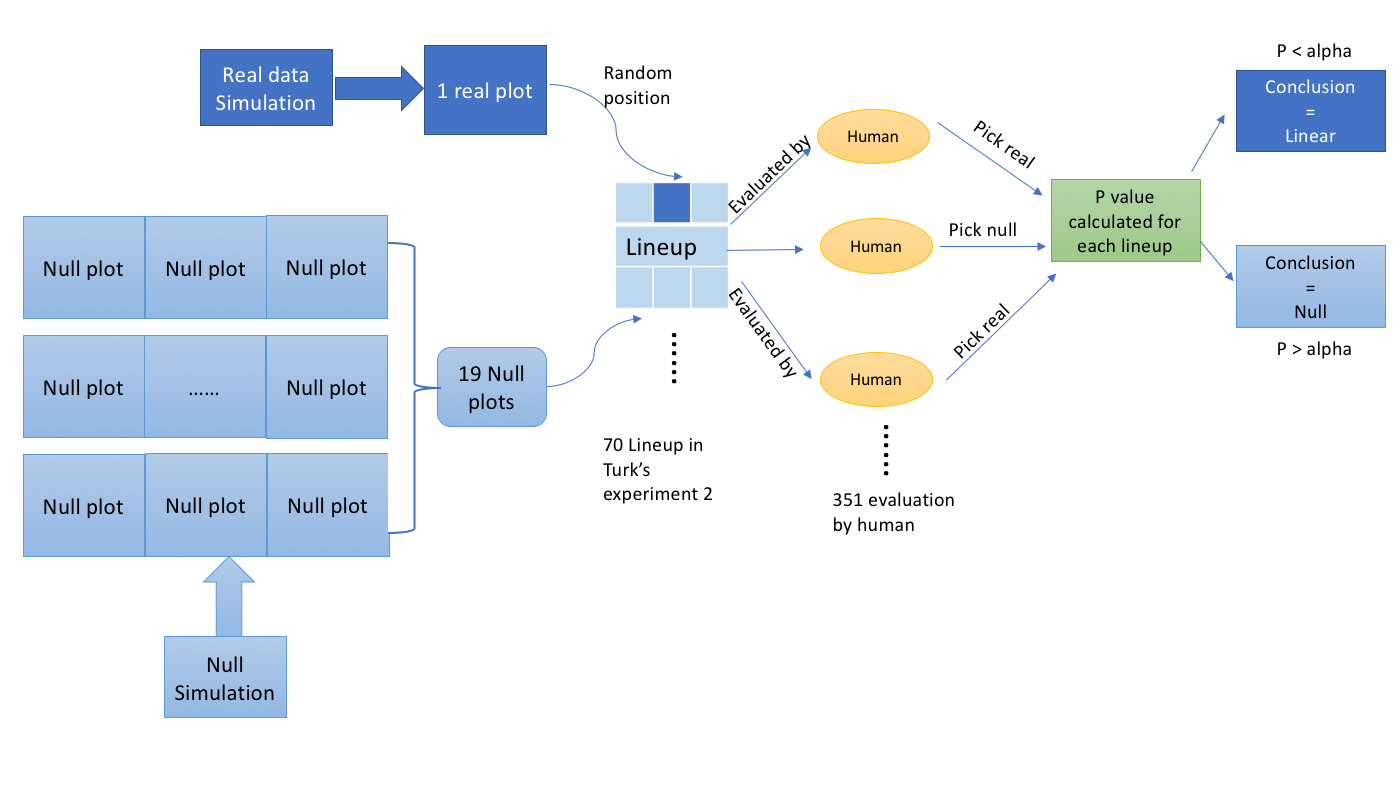
\includegraphics[width=15cm]{figures/diaghm.png}}
\caption{Diagram illustrating the process of human subject evaluation of lineups, and how performance is computed.}
\label{dghm}
\end{figure*}

\bibliographystyle{agsm}
\bibliography{bibliography.bib}

\end{document}
